% !TeX program = lualatex
% !TeX encoding = UTF-8
% !TeX spellcheck = pt_BR
\documentclass[10pt, hyperref={pdfpagelabels=false}]{beamer}
\usepackage[utf8]{inputenc}
\usepackage[brazil]{babel}
\usepackage{lmodern}
\usepackage{url}
\usepackage{csquotes}

% Permite colocar figuras lado a lado ou
% fazer posicionamentos arbitrários
%\usepackage[lofdepth,lotdepth]{subfig}

% Para inserir gráficos e imagens
\usepackage{graphicx}
% Diretório padrão para figuras
\graphicspath{ {images/} }

% Para poder fazer texto cortado (strikethrough)
\usepackage[normalem]{ulem}

\usetheme[progressbar=frametitle]{metropolis}
\usepackage{appendixnumberbeamer}

\usepackage{booktabs}
\usepackage[scale=2]{ccicons}

\usepackage{pgfplots}
\usepgfplotslibrary{dateplot}

\usepackage{xspace}
\newcommand{\themename}{\textbf{\textsc{metropolis}}\xspace}

% Notações matemáticas usadas na dissertação.
% Usando elas é possível trocar toda a notação
% apenas mexendo nesse arquivo. Lembre sempre
% de olhá-lo antes de fazer equações.
% Para fórmulas matemáticas
\usepackage{amsmath}
\usepackage{amssymb}
\usepackage{mathtools}

% Para setas usadas em fórmulas dos grafos
\usepackage{MnSymbol}

% Notações matemáticas usadas com frequência no texto.
% Isso possui três vantagens:
% 1 - Dá menos trabalho digitar as fórmulas
% 2 - Dá mais consistência à notação no trabalho
% 3 - Se mudar de ideia qto à notação, é só trocar aqui
%     e o trabalho todo fica certo.
% Notação matemática
\newcommand{\R}{\mathbb{R}} % Reais
\renewcommand\vec{\mathbf} % vetor como negrito
\newcommand{\avg}[1]{\left\langle #1 \right\rangle} % ... média
\newcommand{\defn}{\coloneqq} % Usamos "=", ":=" ou "\equiv?"
\newcommand{\noloop}[1]{#1^\nlcirclearrowleft} % ... sem loops
% Redes direcionadas
\newcommand{\linkin}[1]{#1^\leftarrow} % ... entrada
\newcommand{\linkout}[1]{#1^\rightarrow} % ... saída
\newcommand{\linkboth}[1]{#1^\leftrightarrow} % ... direcionada
% Redes ponderadas e direcionadas
\newcommand{\win}{w^\leftarrow} % peso e direção de entrada
\newcommand{\wout}{w^\rightarrow} % peso e direção de saída
\newcommand{\weighted}[1]{#1^w} % ... com pesos
\newcommand{\weighteddir}[1]{#1^{w\rightarrow}} % ... com peso e direção
% Reciprocidade
\newcommand{\recin}[1]{#1^\leftlsquigarrow} % ... entrada não-recíproca
\newcommand{\recout}[1]{#1^\leadsto} % ... saída não-recíproca
\newcommand{\recboth}[1]{#1^\leftrightsquigarrow} % ... recíproca
% Capacidades
\newcommand{\capac}{\textit{cap}}

\title{Qualificação}
\subtitle{Um Estudo do Mapa de Carreiras da Empresa Vagas.com Usando Ciência de Redes}
% \date{\today}
\date{}
\author{Aluno: Ronie Uliana \\ Orientador: Prof. Dr. Leandro Nunes de Castro}
\institute{Universidade Presbiteriana Mackenzie}
% \titlegraphic{\hfill\includegraphics[height=1.5cm]{logo.pdf}}

\begin{document}

\maketitle

\begin{frame}{Conteúdo}
  \setbeamertemplate{section in toc}[sections numbered]
  \tableofcontents[hideallsubsections]
\end{frame}

%===================
\section{Introdução}
%===================

\begin{frame}[fragile, label=pessoas]{Pesquisador e o Orientador}

  \begin{alertblock}{Ronie Uliana}
    Mestrando, Mackenzista, ex-UNAERP, ex-VAGAS.com, 99ner, Arquiteto de Software, \textit{Aluno}.
  \end{alertblock}
  
  \begin{alertblock}{Prof. Doutor Leandro de Castro}
    Doutor, Mackenzista, Pai, referência em Computação Natural, Empreendedor, \textit{Orientador}.
  \end{alertblock}
\end{frame}

\begin{frame}[fragile, label=pesquisa]{A Pesquisa}
  \begin{center}
    Uma \alert{análise de dados exploratória}\\
    sobre movimentação de profissionais entre ocupações\\
    utilizando técnicas de \alert{Ciência de Redes}\\
    sobre a base de currículos da empresa VAGAS.com
  \end{center}
\end{frame}

\begin{frame}[fragile, label=objetivo]{Objetivo}
  \begin{center}
    Encontrar e propor \alert{hipóteses} plausíveis\\
    sobre movimentação profissional
  \end{center}
\end{frame}

\begin{frame}[fragile, label=dados]{Dados}
  Currículos anonimizados da empresas VAGAS.com (Fevereiro/2017).
  
  \begin{itemize}
    \item 10 milhões de currículos;\\
    \item 23 milhões de experiências profissionais;\\
    \item 8.348 ocupações distintas.
  \end{itemize}
\end{frame}

%=========================
\section{Ciência de Redes}
%=========================

{
\setbeamercolor{background canvas}{bg=white}
\begin{frame}[label=conceitos-basicos]{Conceitos de Redes}
  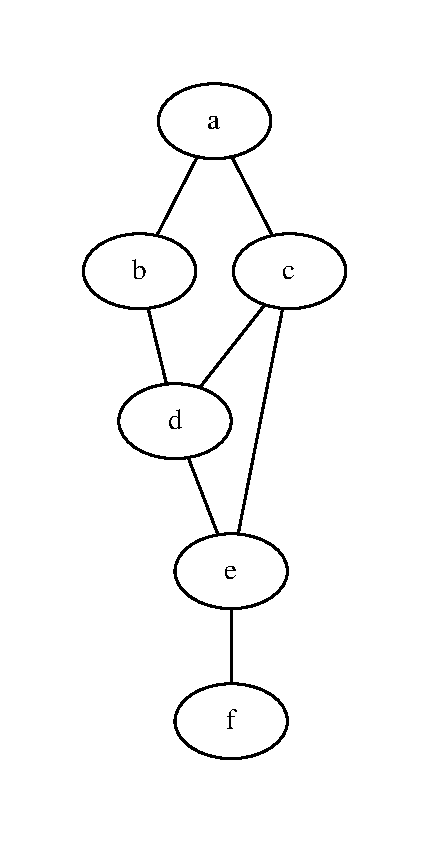
\includegraphics[width=0.2\textwidth]{simple.pdf}
  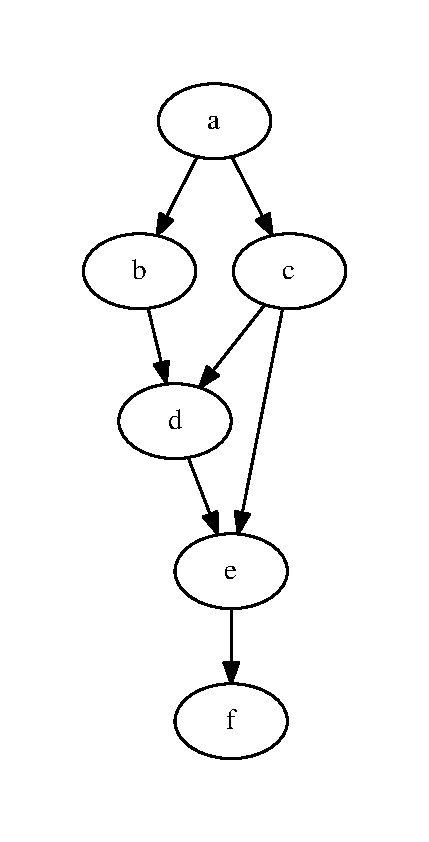
\includegraphics[width=0.2\textwidth]{directed.pdf}
  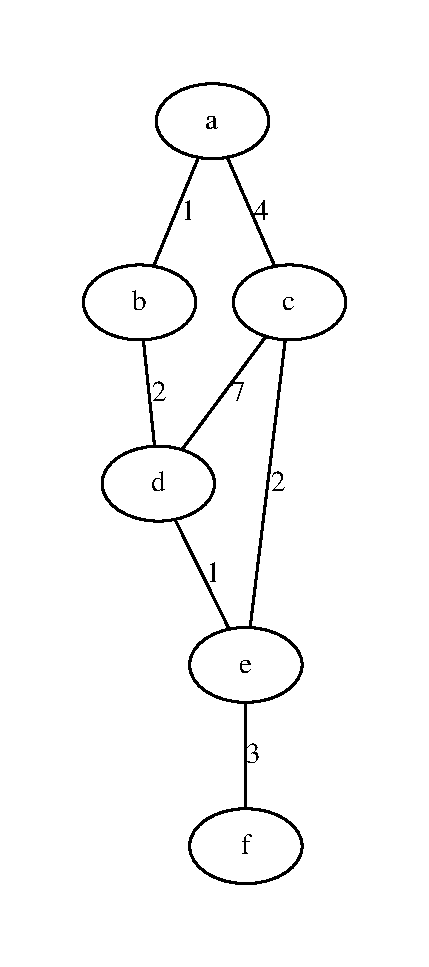
\includegraphics[width=0.2\textwidth]{weighted.pdf}
  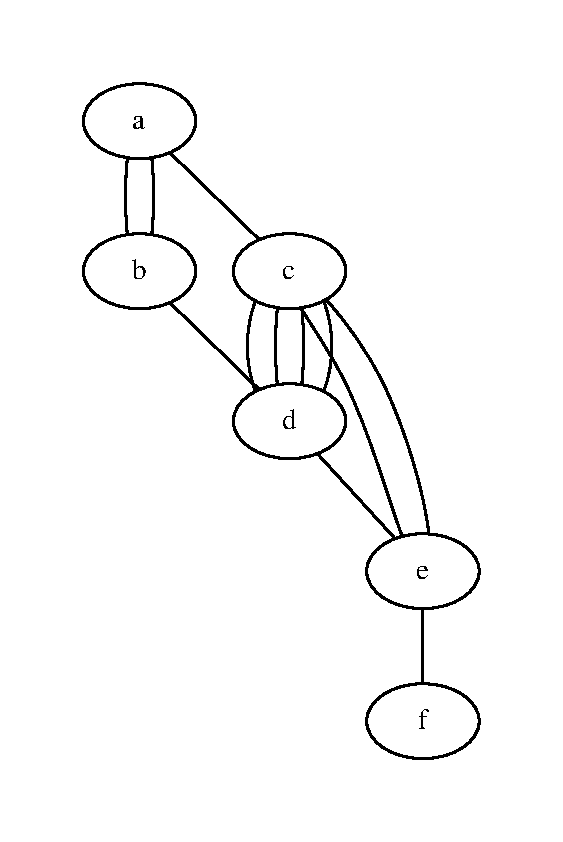
\includegraphics[width=0.2\textwidth]{multiple.pdf}
  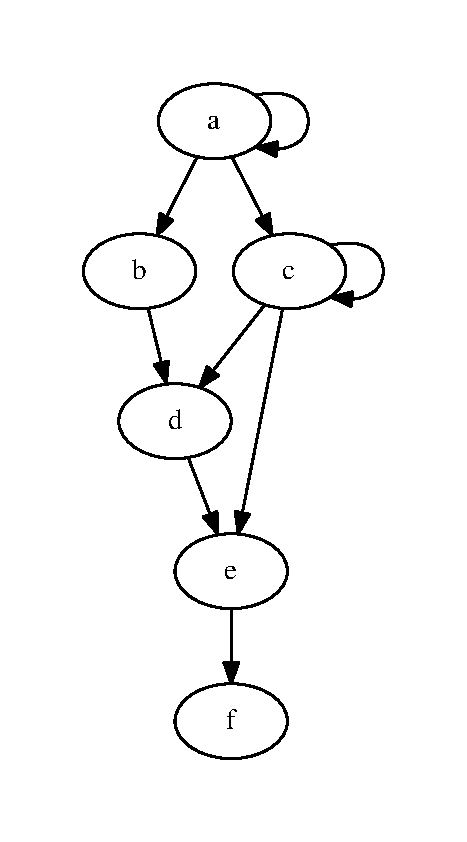
\includegraphics[width=0.2\textwidth]{loop.pdf}
\end{frame}
}

\begin{frame}[label=historia]{Breve História}
  \begin{itemize}
    \item Teoria de Grafos (Euler, século 18) - Matemática;
%    \item Redes Aleatórias (Erdős-Rényi/Gilbert, 1958) - Análise Combinatória e Estatística;
    \item Mundo Pequeno (Watts-Strogatz, 1998) - Popularização;
    \item Livre de Escala (Barabási-Albert, 1999) - Redes Complexas;
    \item Reconhecimento (USNRC, 2005) - \alert{Ciência de Redes}.
  \end{itemize}
\end{frame}

\begin{frame}[label=definicao]{Definição}
  National Research Council (2006)~\cite{National_Research_Council2006-lv}:
  \begin{quote}
    O estudo da representação em rede de fenômenos físicos, biológicos e sociais levando a modelos preditivos desses fenômenos.
  \end{quote}
  Barabási e Pósfai (2016)~\cite{Barabasi2016-rn}:
  \begin{itemize}
    \item Interdisciplinar;
    \item Empírica;
    \item Matemática e Quantitativa;
    \item Computacional;
  \end{itemize}
\end{frame}

\begin{frame}[label=redes]{Redes Aleatórias e Redes Reais}
Redes aleatórias são \alert{Modelos Nulos}, similares à hipótese nula em estatística.

Se uma característica observada em uma \alert{Rede Real} não aparece em uma \alert{Rede Aleatória} equivalente, deve existir um \alert{princípio organizacional} ausente no Modelo Nulo.
\end{frame}

\begin{frame}[label=medidas]{Medidas}
  O que caracteriza uma rede:
  \begin{itemize}
    \item Grau e Força;
    \item Distância Geodésica;
    \item Centralidade;
    \begin{itemize}
      \item Grau e Força;
      \item Intermediação;
    \end{itemize}
    \item Coeficiente de Agrupamento;
    \item Reciprocidade;
    \item Assortatividade, similaridade, modularidade.
  \end{itemize}
\end{frame}

\begin{frame}[label=propriedades]{Propriedades Topológicas}
  \begin{alertblock}{Mundo Pequeno}
    A distância geodésica esperada entre dois nós quaisquer é muito pequena.
  \end{alertblock}
  \begin{alertblock}{Livre de Escala}
    A rede possui poucos nós muito conectados (\textit{hubs}) e muitos nós pouco conectados.
  \end{alertblock}
\end{frame}

\begin{frame}[label=modelos-nulos]{Modelos Nulos}
  Algoritmos para geração de redes aleatórias com características específicas para serem \alert{Modelos Nulos}.
  \begin{description}
    \item[Erdős-Rényi/Gilbert] Base do modelo aleatório;
    \item[Preservação de Grau] Preserva o grau de cada nó;
    \item[Preservação de Força] Preserva a força de cada nó\footnote{Contribuição do autor};
    \item[Xulvi-Brunet e Sokolov] Assortatividade artificial.
    \item[Randomização de Força] Desassociação de força e grau\footnote{Contribuição do autor (em desenvolvimento)}.
  \end{description}
\end{frame}

\section{Mapa de Carreiras}

{
\setbeamercolor{background canvas}{bg=white}
\begin{frame}[label=mapa-visao-geral]{Visão Geral}
  \begin{center}
    Um grafo resumindo a trajetória profissional\\dos usuários do site VAGAS.com.br

    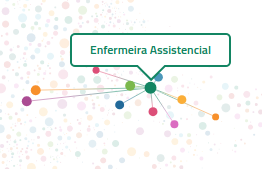
\includegraphics[width=0.4\textwidth]{mapa-enfermeira-assistencial}

  Cerca de \alert{10 milhões} de usuários\\resultando em \alert{8.348 ocupações} conectadas
  \end{center}
\end{frame}
}

\begin{frame}[label=mapa-construcao]{A Construção}
  \begin{center}
    Pipeline
    
    Processamento de texto
    
    Agrupamento de dados por ocupação
  \end{center}
\end{frame}

{
\setbeamercolor{background canvas}{bg=white}
\begin{frame}[label=mapa-dados]{Os Dados}
  Os dados disponíveis:

  \begin{columns}[T,onlytextwidth]
    \begin{column}{0.5\textwidth}
      \begin{itemize}
        \item Fluxo de profissionais
        \item Salários
        \item Tempo de Permanência
        \item Graduações
        \item Palavras-chave
      \end{itemize}
    \end{column}
    
    \begin{column}{0.5\textwidth}
      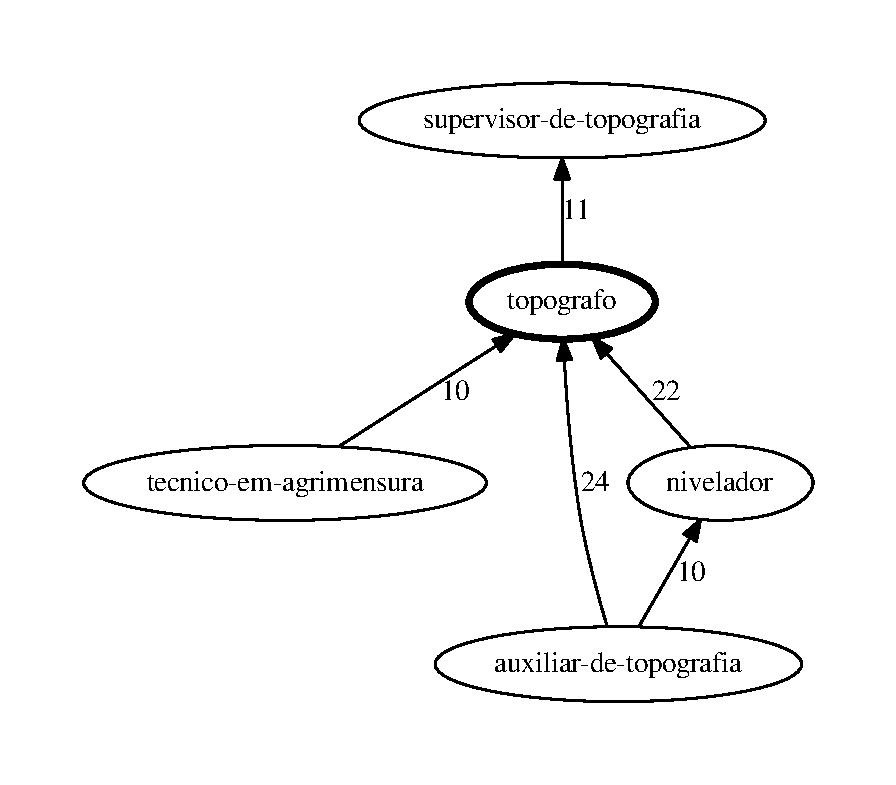
\includegraphics[width=\textwidth]{cluster_25}
    \end{column}
  \end{columns}
\end{frame}
}

\section{Resultados Parciais}

\begin{frame}[label=hipoteses]{As Hipóteses}
  \begin{enumerate}
    \item \alert{Atração Profissional}
    \item \sout{Correlação Negativa entre Força de Entrada e a Mediana Salarial}
    \item \alert{Pontos de Saída do Mercado de Trabalho}
    \item \alert{Pontos de Entrada do Mercado de Trabalho}
    \item Trabalhos de Passagem
    \item Equivalência Profissional 
    \item Detecção de Nomenclatura Equivalente 
    \item \alert{Capacitação Parcial}
    \item \alert{Identificação de Carreiras}
  \end{enumerate}
\end{frame}

\begin{frame}[c, label=hipotese-atracao]{Hipótese 1: Atração Profissional}
  \begin{center}
    \begin{columns}[T,onlytextwidth]
      \begin{column}{0.4\textwidth}
        Ordem por força de \alert{saída} da ocupação.
        
        \begin{center}
        \includegraphics[height=0.4\textheight]{preferencia-de-atracao}
        \end{center}
         
        Mediana da ordem na ocupação de \alert{entrada}.
        
      \end{column}
      \begin{column}{0.6\textwidth}
        \centering
        \footnotesize
        \begin{table}[!h]
          \centering
          \begin{tabular}{l|r|r}
            \hline
            Ocupação & Pos & Entre\\
            \hline
            administrativo auxiliar & 2 & 2591\\
            \hline
            administrativo assistente & 4 & 1694\\
            \hline
            vendedor & 4 & 1553\\
            \hline
            recepcionista & 4 & 1176\\
            \hline
            auxiliar producao & 5 & 885\\
            \hline
            atendimento & 7 & 904\\
            \hline
            enfermeiro & 1 & 121\\
            \hline
            caixa operador & 7 & 745\\
            \hline
            analista sistema & 3 & 300\\
            \hline
            motorista & 7 & 547\\
            \hline
          \end{tabular}
        \end{table}
      \end{column}
    \end{columns}
  \end{center}
\end{frame}

\begin{frame}[c, label=hipotese-salario]{Hipótese 2: Correlação entre Salário e Força de Entrada}
  \begin{center}
    Hipótese \alert{refutada}
    
    Correlação $\approx 0,98$ entre força de entrada e saída
    
    Correlação $> 0,95$ entre todos os graus e forças
  \end{center}
\end{frame}

{
\setbeamercolor{background canvas}{bg=white}
\begin{frame}[c, label=hipotese-salario-graduacao]{Hipótese 2 (alternativa): Correlação entre Salário e Graduação}
  \begin{center}
    \begin{columns}[onlytextwidth]
      \begin{column}{0.5\textwidth}
        \centering
        Não há uma correlação linear
        
        \vspace{\baselineskip}
        
        3º Quartil
        
        2.000 ou 4.000
        
        \vspace{\baselineskip}
        
        Ensino Médio $> 4.000$
        
        \vspace{0.5\baselineskip}
        
        \tiny
        \begin{table}[!h]
          \begin{tabular}{l|r|r}
            \hline
            Ocupação & Sal & Prof\\
            \hline
            \alert{cabotagem mestre} & 8.137 & 46\\
            \hline
            mestre obra & 4.925 & 315\\
            \hline
            conves marinheiro & 4.495 & 275\\
            \hline
            maquina marinheiro & 4.314 & 107\\
            \hline
            aeronaves manutencao tecnico & 4.117 & 205\\
            \hline
            preditivo tecnico & 4.006 & 50\\
            \hline
          \end{tabular}
        \end{table}
      \end{column}
      
      \begin{column}{0.5\textwidth}
        \includegraphics[width=0.9\textwidth]{salario-por-graduacao}
      \end{column}
    \end{columns}
  \end{center}
\end{frame}
}

{
  \setbeamercolor{background canvas}{bg=white}
\begin{frame}[c, label=hipotese-pontos-entrada-e-saida]{Hipóteses 3 e 4: Pontos de Entrada e Saída}
  \begin{center}
    \begin{columns}[onlytextwidth]
      \begin{column}{0.5\textwidth}
        Variação da equação de reciprocidade:
        
        \begin{equation*}
          \recboth{s_i} \defn \frac{\linkin{s_i} - \linkout{s_i}}{s_i}
        \end{equation*}
        
        \begin{itemize}
          \item[] $s_i$ força do nó $i$
          \item[] $\linkin{s_i}$ força de entrada
          \item[] $\linkout{s_i}$ força de saída
        \end{itemize}
      \end{column}
    
      \begin{column}{0.5\textwidth}
        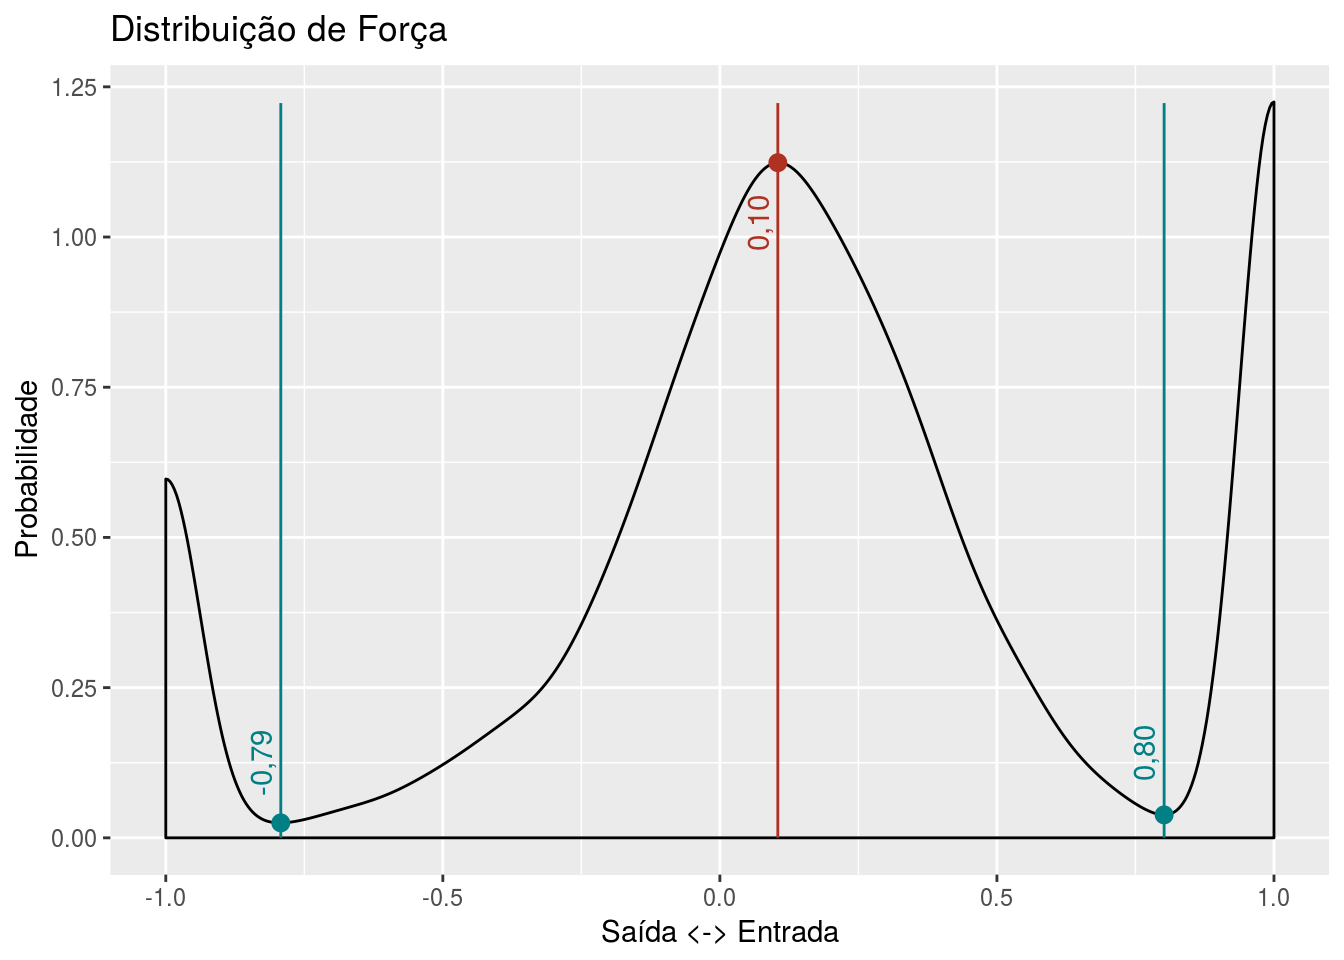
\includegraphics[width=\textwidth]{distribuicao-de-forca}
      \end{column}
    \end{columns}
  
    \vspace{\baselineskip}
  
    \textbf{-1} significa \enquote{somente saída} e \textbf{1} significa \enquote{somente entrada}
  \end{center}
\end{frame}
}

\begin{frame}[label=hipotese-ponto-de-saida-tabela]{Pontos de Saída}
  \begin{center}
    Ocupações com $\recboth{s_i}$ no \textit{limiar de saída}
    
    \vspace{\baselineskip}
    
    \begin{tabular}{l|c|c|c|c}
      \hline
      Ocupação & $s_i$ & $\linkin{s_i}$ & $\linkout{s_i}$ & $\recboth{s_i}$\\
      \hline
      analista desenvolvimento pesquisa & 111 & 101 & 10 & 0.82\\
      \hline
      analista gestao & 113 & 103 & 10 & 0.82\\
      \hline
      analista commerce & 126 & 115 & 11 & 0.83\\
      \hline
      coordenador unidade & 121 & 111 & 10 & 0.83\\
      \hline
      consultor investimento & 152 & 142 & 10 & 0.87\\
      \hline
      fonoaudiologo & 181 & 170 & 11 & 0.88\\
      \hline
    \end{tabular}
  \end{center}
\end{frame}


\begin{frame}[label=hipotese-ponto-de-entrada-tabela]{Pontos de Entrada}
  \begin{center}
    Ocupações com $\recboth{s_i}$ no \textit{limiar de entrada}
    
    \vspace{\baselineskip}
    
    \begin{tabular}{l|r|r|r|r}
      \hline
      Ocupação & $s_i$ & $\linkin{s_i}$ & $\linkout{s_i}$ & $\recboth{s_i}$\\
      \hline
      administrativo aprendiz jovem tecnico & 123 & 10 & 113 & -0.84\\
      \hline
      atendimento cliente profissional & 163 & 14 & 149 & -0.83\\
      \hline
      maquina moco & 138 & 12 & 126 & -0.83\\
      \hline
      embalador repositor & 143 & 13 & 130 & -0.82\\
      \hline
      equipe treinador & 185 & 17 & 168 & -0.82\\
      \hline
      aprendiz jovem mecanico & 135 & 13 & 122 & -0.81\\
      \hline
    \end{tabular}
  \end{center}
\end{frame}

{
\setbeamercolor{background canvas}{bg=white}
\begin{frame}[c, label=hipotese-carreira]{Hipóteses 9 e 8: Identificação de Carreiras}
  \begin{center}
    Se a hipótese 8 está correta,\\detecção de comunidade identifica \alert{carreiras}.
  
    \begin{columns}[T,onlytextwidth]
      \begin{column}{0.5\textwidth}
        \tiny
        \begin{itemize}
          \item[] assistente-tecnico-de-telecomunicacoes
          \item[] auxiliar-tecnico-em-telecomunicacoes
          \item[] consultor-de-telecomunicacoes
          \item[] engenheiro-de-telecomunicacoes
          \item[] especialista-em-telecomunicacoes
          \item[] estagiario-de-telecomunicacoes
          \item[] supervisor-de-telecomunicacoes
          \item[] tecnico-de-dados
          \item[] tecnico-de-implantacao
          \item[] tecnico-de-transmissao
          \item[] tecnico-em-telecomunicacoes
          \item[] tecnico-em-telefonia
          \item[] \alert{tecnico-especialista}
          \item[] tecnico-especialista-em-telecomunicacoes
        \end{itemize}
      \end{column}
      
      \begin{column}{0.5\textwidth}
        \includegraphics[width=\textwidth]{cluster_23}
      \end{column}
    \end{columns}
  \end{center}
\end{frame}
}

\begin{frame}[label=hipoteses-pendentes]{Hipóteses Pendentes}
  \begin{enumerate}
    \setcounter{enumi}{5}
    \item Trabalho de Passagem
    \item Equivalência Profissional
    \item Detecção de Nomenclatura Equivalente
  \end{enumerate}
\end{frame}

\begin{frame}[label=hipoteses-novas]{Novas Hipóteses}
  \begin{enumerate}
    \setcounter{enumi}{10}
    \item Atração por Graduação
    \item Salário por Graduação
    \item Estabilidade de Ocupação
    \item Salário por Estabilidade
  \end{enumerate}
\end{frame}

{
\setbeamercolor{palette primary}{fg=black, bg=yellow}
\begin{frame}[standout]
  Perguntas?
\end{frame}
}

\appendix

\begin{frame}[allowframebreaks]{Referências Bibliográficas}

  \bibliography{main}
  \bibliographystyle{abbrv}

\end{frame}

\end{document}
